\documentclass[12pt]{article}
\usepackage{graphicx}
\usepackage{hyperref}
\usepackage{here}
\usepackage{wrapfig}
\usepackage{lipsum}


% * <prakharguptaiitd@gmail.com> 2016-03-10T14:54:22.944Z:
%
% ^.

\begin{document}
\begin{titlepage}
\title{COP290}
\centering
{\scshape\Large COP290\par}
\vspace{1cm}
{\scshape\Huge GRS - Grievance Resolution System\par}


\vspace{3cm}
  {\Large\itshape Prakhar Agrawal (2014CS10207)\par}
\vspace{0.3cm}
  {\Large\itshape Mayank Rajoria (2014CS10233)\par}
\vspace{0.3cm}
  {\Large\itshape Prakhar Gupta (2014CS10290)\par}


\vfill
\raggedleft
Course  Coordinator\\
Prof. Vinay Joseph Ribeiro
% \vfill
\end{titlepage}

\begin{abstract}
The purpose of this assignment was to create a complaint system for our institute. The main platform decided for this platform is Android for front-end and a Web2Py server for back-end and API. The developed API would be Restful and would easily allow the system to be ported to any platform easily. There will be several levels of complaints allowed and each level shall have its corresponding sub-levels/domains. These shall together decide who has to solve the problem, who can mark it as resolved and who can see he problem. The problems shall have associated statuses with it which can be updated by allowed people and also comments which can be made on the overall complaint or on a particular status of the complaint.
% \vfill
\end{abstract}


% Mention the detailed description of what the application does.

\section{Introduction}
This project aims to make a complaint system for our institute. Using the complaint system, the user shall be able to report complaints at various levels like individual, hostel and institute, direct them to different authorities for solving the problem. The users who can view the problem will also be able to see the latest status of work on the problem along with the history of its status changes. To voice their opinion, users shall be given the option of upvotes/downvotes and comments. This shall allow feedback from community and allow the problem solving to be a more transparent and community driven process.
\par
We shall be developing our back-end in Web2Py and expose the API which can be called by the front-end on any platform. For the first phase of development, we will develop the complaint system on Android. This is keeping in mind that a majority of students on campus use an Android device and having an app on the mobile shall make the complaint registering process convenient. Our API shall adhere to the Restful practices and are designed in such a way that a front-end for it can be developed for any platform with minimal effort and knowledge of back-end. 
\par
We identified that the need of such a system may exists not only in our institute but also in other institute and even in other types of hierarchical settings like offices, societies etc. Keeping this in mind we have developed our database in such a way that it allows flexibility. To use the complaint system in any other place, only the entries in certain tables of the database shall need to be changed. The tables, API, front-end can remain exactly the same.

\section{Complaint Life-cycle}
\begin{itemize}
\setlength\itemsep{-0.4em}
\item The complaint is made my a user wherein he describes the level, domain and details of the complaint.
\item The Users/Groups responsible for solving the complaint and the Users/Groups who can see the complaint are added based on the level and domain of the complaint.
\item Additionally more people can be given the right to mark complaint as resolved by the user, for example I may want my room mate to be able to mark the complaint as resolved once the tube light of our room is fixed.
\item The complaint status can be updated with custom text by the person responsible for solving the complaint or whoever has the permission to mark it as resolved.
\item Predefined complaint status like "Work started" ,"Solved", "Resolved" and "Complaint forwarded" are also provided.
\item Users who can view the complaint can comment on individual status and on overall complaint too.
\item Each complaint shall have upvote and downvote buttons to allow a simple way for people to express their opinion.
\item Complaint may also be bookmarked by users if they want to receive notifications about its status change and shall also be marked as "read" on server once the user has seen the complaint after latest status change.
\item Complaint would be considered solved only after the person with rights to update its status as resolved has done so.
\end{itemize}


\section{User Interface - Android Client Mockup}
\par
UI is planned out to be a complete swap/swipe based UI. The mockups presented below only represent the user/complaint information to be received/displayed. It is a rough representation of how application space can be used without crunching lots of information into too little space. Andorid Client for the web application has been made fully sufficient with all functionality that the web interface provides. GRS will be divided into a large range of activities for easier user navigation and handling
\begin{itemize}
  \item Login/Signup
  \item Complaint Lodge
  \item View Complaints Affecting You
  \item View Complaints you have received
  \item View Bookmarked Complaints
  \item View Notifications
  \item View User Profile
  \item Validation Requests from others
  \item Complaint Description
      \begin{itemize}
      \item Complaint Timeline
          \item Complaint Wall
    \end{itemize}
    
\end{itemize}


    \subsection{GRS Main Screen}
    \par
    Figure \ref{fig:appFrontScreen} is the opening screen of the application. If the user is not already logged in he is auto directed to login activity otherwise he is directly taken to the Main Application activity as shown in Figure \ref{fig:complainAffectingYouScreen} . Figure \ref{fig:loginScreen} is the login screen where the user enters his username and password to access the application interface. We plan to integrate the complaint System with the LDAP user profiles and authenticate the user via the LDAP-Kerberos used at IIT Delhi. This in the long run will enable us to integrate the user and their workgroup directly from the IIT Delhi database avoiding the redundancies of the registration or the signup process.



    \begin{figure}[H]
    \begin{minipage}{.5\textwidth}
      \centering
      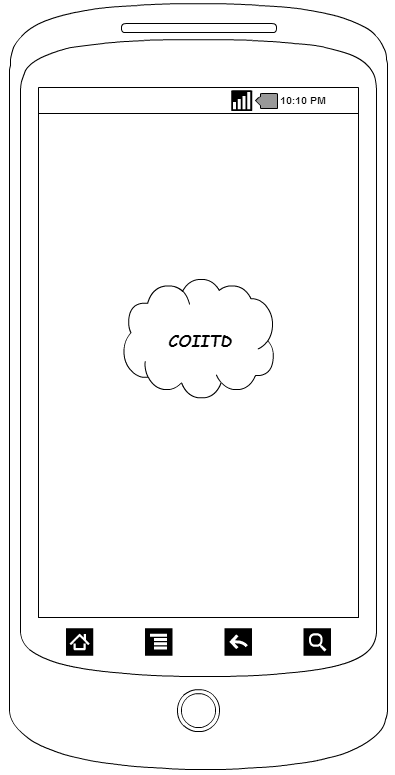
\includegraphics[width=0.9\textwidth]{./appMockUp/appFrontScreen}
      \caption{App Front Screen}
      \label{fig:appFrontScreen}
    \end{minipage}%
    \begin{minipage}{.5\textwidth}
      \centering
      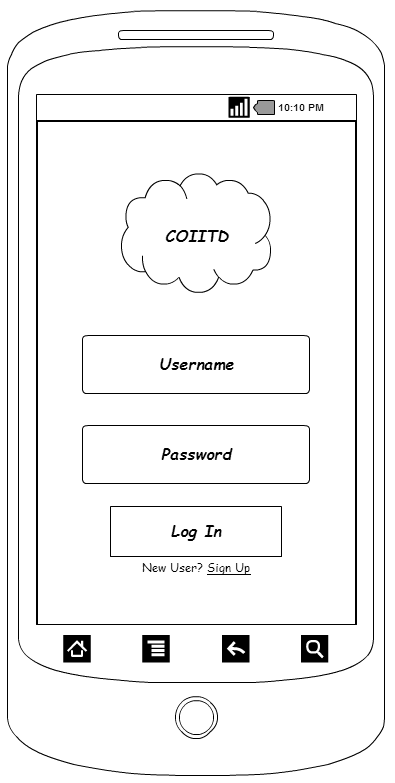
\includegraphics[width=0.9\textwidth]{./appMockUp/loginScreen}
      \caption{Login Screen}
      \label{fig:loginScreen}
    \end{minipage}

    \end{figure}



    % \begin{figure}[H]
    %     \hspace*{-0.75 in}
    %   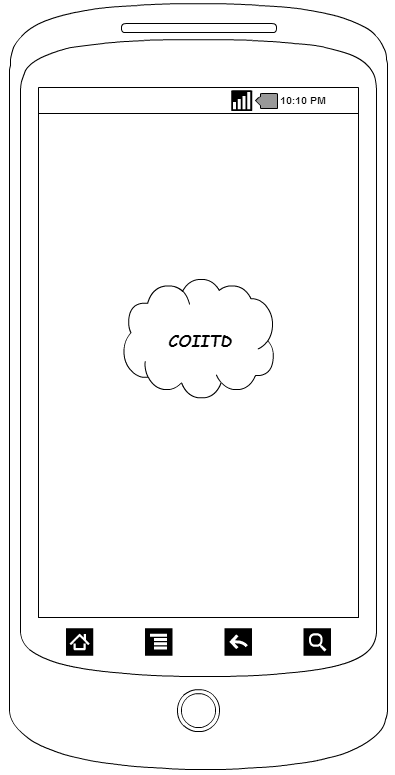
\includegraphics[width=0.5\textwidth]{./appMockUp/appFrontScreen}
    %   \label{fig:appFrontScreen}
    %     \hspace*{0.75 in}
    %     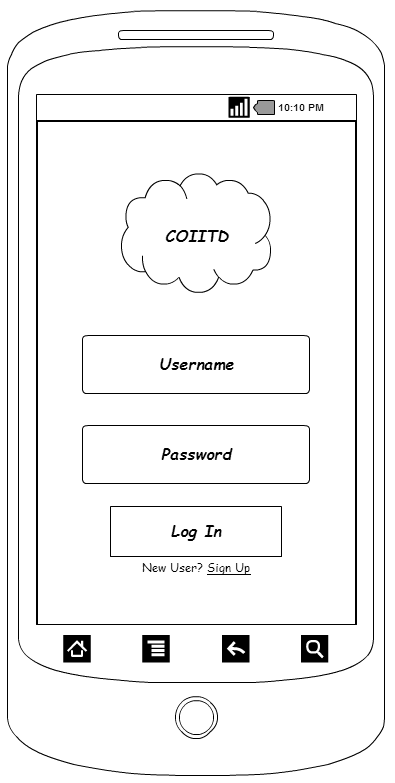
\includegraphics[width=0.5\textwidth]{./appMockUp/loginScreen}
    %   \label{fig:loginScreen}
    %   \caption {(a) Front Screen     (b) Login Screen}

    % \end{figure}


    \subsection{Sign Up Screen}
    \par 
    \begin{itemize} 
    \item The Sign up activity has been added as a fallback for an institution that lacks user database or a common authentication APIS. 
    \item User is allowed to enter all his workgroups for which he is responsible and answerable to the institution or the company.
    \item Care has been taken to not allow users to directly enter any group or subgroups in the backend by setting a validation flag to \textit{false}.
    \item This temproary screen can be easily disabled by just removing the singly provided link on the startup activity and \textbf{\textit{disabling the signup API}}
    \end{itemize}


    \begin{figure}[H]
        \centering
        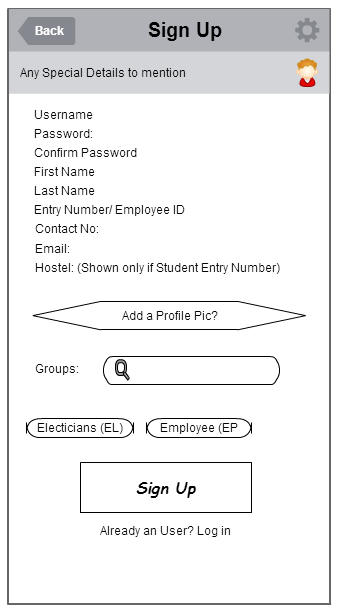
\includegraphics[width=0.5\textwidth]{./appMockUp/signUpScreen}
        \label{fig:SignUpScreen}
        \caption{Sign Up Screen}

    \end{figure}




  
    \subsection{Main Activity}
    \subsubsection{Complaints Concerning User - Fragment 1}
    \par 
    \begin{itemize} 
    \item This \ref{fig:complaintsAffectingYouScreen} screen shows the current user any \textbf{\textit{complaints directly or indirectly affecting the current user}}.
    \item Complaints affecting the user and those that come to the current user have been wisely separated out in this fragment and the following fragment as shown in via the figures \ref{fig:complaintsAffectingYouScreen} and \ref{fig:othersComplaintsScreen}
    \item Each complaint listed in the figure has a \textbf{complaint title, Associated description in short, Complaint Pic (if available), Complaint Level Indicated by the diamond coloured according to a level, a bookmark status and a upvote/downvote count}
    \item Each complaint can be swiped left to view more options corresponding to the complaint such as \textbf{\textit{Hide the complaint, Bookmark the complaint, etc}}.
    
    \end{itemize}


    \begin{figure}[!ht]
      \begin{minipage}{.5\textwidth}
        \centering
        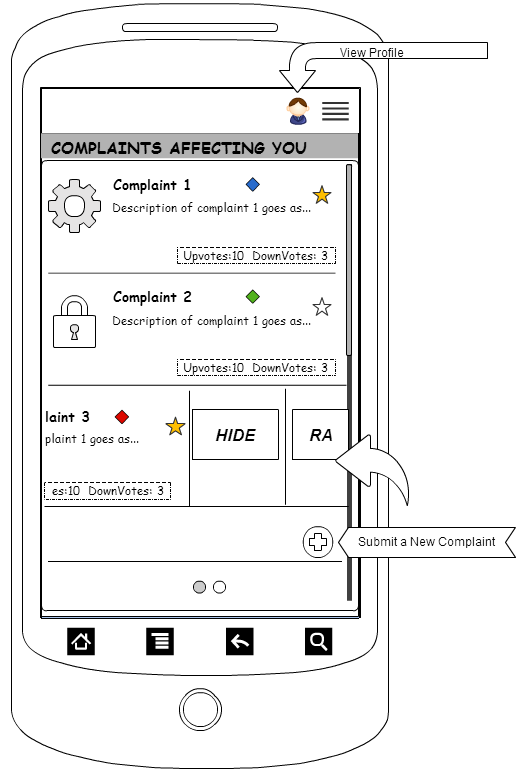
\includegraphics[width=1.1\textwidth]{./appMockUp/complaintsAffectingYouScreen}
        \caption{Complaints Concerning Current User}
        \label{fig:complaintsAffectingYouScreen}
      \end{minipage}
      \begin{minipage}{.49\textwidth}
        \centering
        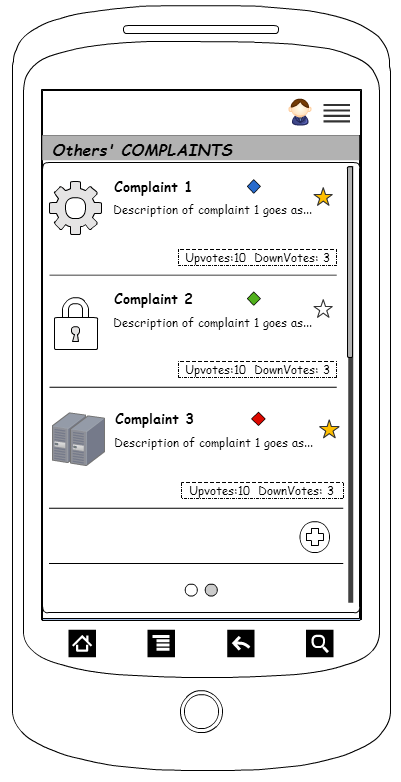
\includegraphics[width=0.84\textwidth]{./appMockUp/othersComplaintsScreen}
        \caption{Complaints addressed to Current User}
        \label{fig:othersComplaintsScreen}
      \end{minipage}

    \end{figure}
      
    \subsubsection{Complaints Addressed to User - fragment 2}
    \par 
    \begin{itemize} 
    \item This Figure \ref{fig:othersComplaintsScreen} screen shows the current user any \textbf{\textit{complaints directly or indirectly addressed to the current user}}.
    \item This part of the fragment can be easily swipe opened by swiping the frame \ref{fig:complaintsAffectingYouScreen} to the left to open up the new fragment.
    \item The \textbf{\textit{Avatar}} on the top right in the action bar is a button to open the profile page which has been shown and described in the sections on profile. Reference Figure %\ref{fig:profileScreen}
    \end{itemize}
    
    
    
    
      
    \subsection{Action Bar Functionality}
     \par 
 %    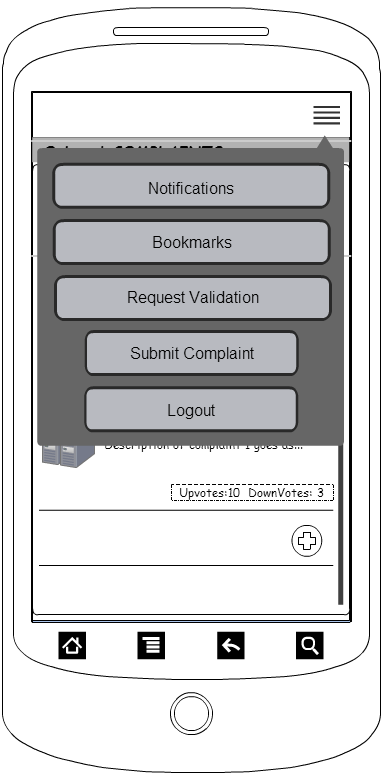
\includegraphics[width=5.5cm]{./appMockUp/actionBarNotificationScreen1}
    \begin{itemize} 
    \item The action bar of the \textbf{Android Client} is designed to include a lot of the application functionality.        

    \item On clicking more on the action bar the user is presented with a variety of buttons such as
      \begin{itemize}
      \item Notifications
            \item Bookmarks
            \item Requests for validation
            \item Submit A Complaint
            \item Logout            
      \end{itemize}
    \item All these buttons may have a slightly different view in the original application but the mockup gives a basic idea of how these components can be arranged.
    \end{itemize}
    
    \begin{figure}[H]
      \centering
    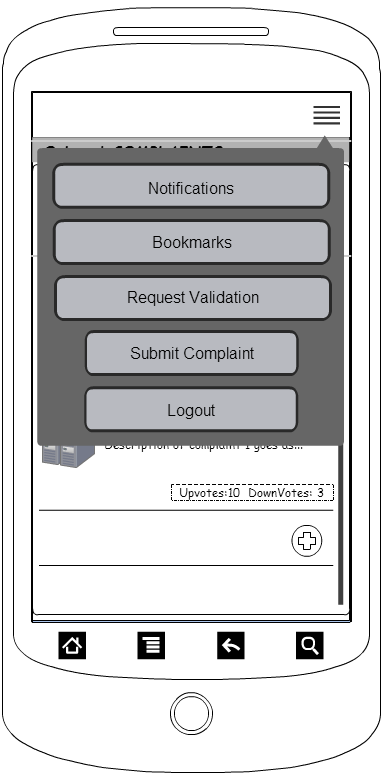
\includegraphics[width=5.5cm]{./appMockUp/actionBarNotificationScreen1} 
      \caption{Action Bar functionality}
        \label{fig:actionBarNotificationScreen1}
     \end{figure}
    
    
    

  
    \subsection{Notifications and Bookmark}
     \par 

    \begin{itemize} 
    \item The simple interface mockups for the notifications and the application Bookmarks (i.e. bookmarked complaints) has been shown in the Figure \ref{fig:notificationsScreen} and the Figure \ref{fig:bookmarksScreen} respectively.
    \item These provide the end user a friendly environment to navigate through the active complaints and the complaints of importance i.e. the ones that are bookmarked by him.
    \end{itemize}
    
     \begin{figure}[!ht]
      \begin{minipage}{.5\textwidth}
        \centering
        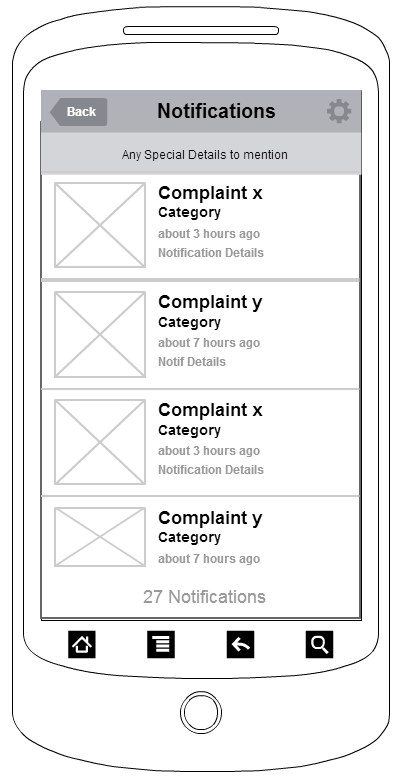
\includegraphics[width=0.9\textwidth]{./appMockUp/notificationsScreen}
        \caption{Notifications Screen}
        \label{fig:notificationsScreen}
      \end{minipage}
      \begin{minipage}{.5\textwidth}
        \centering
        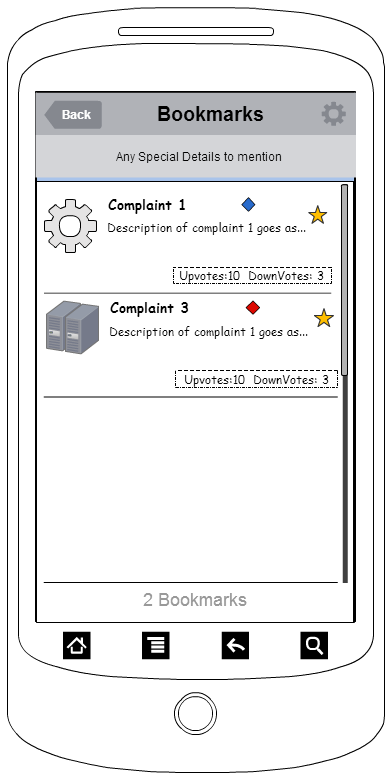
\includegraphics[width=0.9\textwidth]{./appMockUp/bookmarksScreen}
        \caption{Bookmarks Screen}
        \label{fig:bookmarksScreen}
      \end{minipage}

    \end{figure}
    



 \subsection{Profile, Lodge a Complaint, Validation Requests}
     \par 
    \begin{itemize} 
    \item The application mockups for the above mentioned pages have been kept simple in the mockups but may exceedingly use swipe based User Interface that turns the Android application client attractive.
    \item These sections have been shown as in the order above in the Figure \ref{fig:profileScreen}, \ref{fig:submitComplainScreen} and \ref{fig:validationRequestScreen}
    \end{itemize}
    
     \begin{figure}[!ht]
      \begin{minipage}{.32\textwidth}
        \centering
        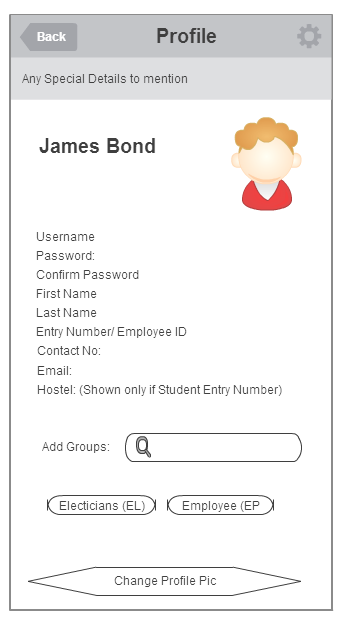
\includegraphics[width=0.9\textwidth]{./appMockUp/profileScreen}
        \caption{User Profile}
        \label{fig:profileScreen}
      \end{minipage}
      \begin{minipage}{.32\textwidth}
        \centering
        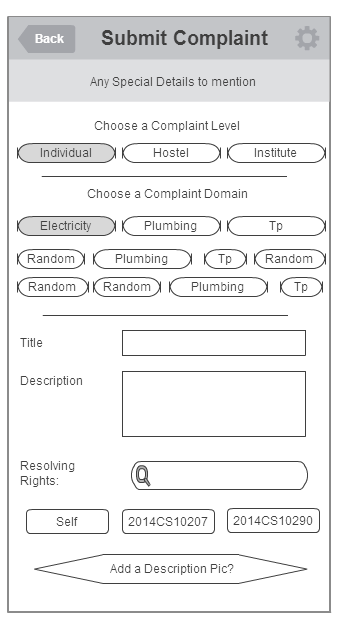
\includegraphics[width=0.9\textwidth]{./appMockUp/submitComplainScreen}
        \caption{Complaint Lodge}
        \label{fig:submitComplainScreen}
      \end{minipage}
      \begin{minipage}{.32\textwidth}
        \centering
        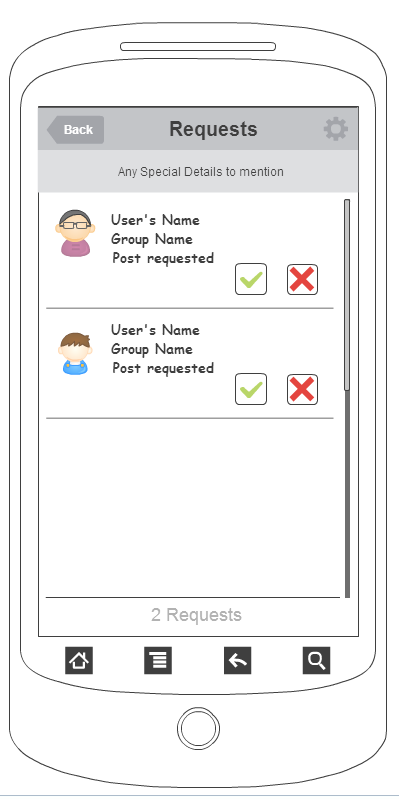
\includegraphics[width=0.85\textwidth]{./appMockUp/validationRequestScreen}
        \caption{Validation Requests}
        \label{fig:validationRequestScreen}
      \end{minipage}

    \end{figure}
    
    


 \subsection{Complaint Description}
     \par The most important part of the application i.e. \textbf{Complaint} itself has been detailed and described in a very user friendly manner. Each complaint has a corresponding description that can be accessed by clicking on the complaint or the complaint notifications as shown in the notifications Figure \ref{fig:notificationsScreen} 
     \par On clicking any complaint the android client opens up a long complaint description Screen that includes complaint title, complaint description, total upvotes/downvotes, Bigger picture related to complaint, complaint current status, whether it has been undertaken by anyone, date undertaken on, posted by, posted on, Complaint location (if relevant) and numerous other details.  
     
     \subsubsection{COMPLAINT TIMELINE}
     \par We plan to describe complaint as a series of progress or changes in the complaint status and we thereby invoke and introduce the concept of \textbf{\textit{"COMPLAINT TIMELINE"}}. Complaint Timeline is chronological display of the progress or significant events in the life cycle of a particular complaint. These events create notifications that are displayed to users that follow/bookmark the complaint to watch it closely.  
     \par We believe in taking righteous opinions of several people over each event in the lifecycle of the complaint and hence we have a comment box and a comment thread relating to each event in the Complaint life cycle.  
 \begin{wrapfigure}{r}{8cm}
  \caption{Complaint Timeline}\label{fig:complainTimelineScreen}
  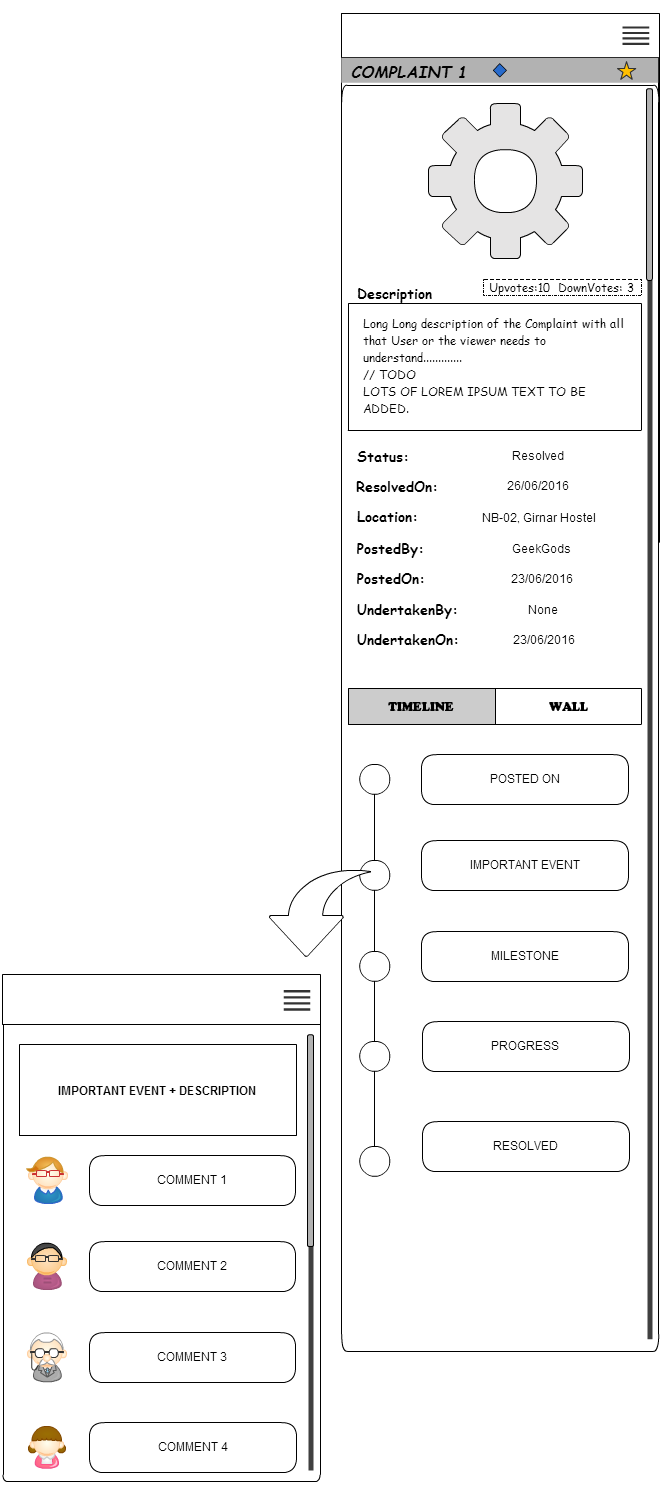
\includegraphics[width=8cm]{./appMockUp/complainTimelineScreen}
  \end{wrapfigure}
    
 \par   The mockup for the above mentioned timeline has been kept simple and is shown in the figure alongside. The comment section for each event in lifecycle is as shown in the figure by a protruding arrow outside the figure in \ref{fig:complainTimelineScreen}. 
 
 
      \subsubsection{COMPLAINT WALL}
      
\par The other tab beside the timeline tab in the complaint description view is of complaint wall, where user/users/resolvers/solvers all can post their opinion, view comments regarding any particular complaint.
 \par This can be used for any number of comments by any user who can view the complaint. This helps in understanding the opinion of the people on widely affecting complaints such as the LAN BAN complaint and giving specific comments in case of the smaller complaints such as that of the tube light and plumbing for an individual hostelite or faculty member.
  
  
  
  %Line breaks
%  \\ \\ \\ \\ \\ \\ \\ \\ \\ \\ \\ \\

    
 \begin{figure}[H]
  \centering
  \caption{Complaint Wall}\label{fig:complaintWallScreen1}
  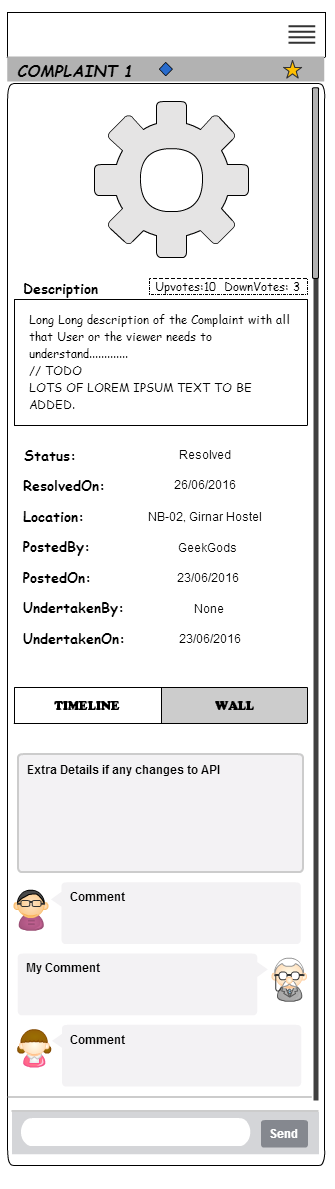
\includegraphics[width=5cm]{./appMockUp/complaintWallScreen1}
  \end{figure}
  
  








\subsection{Deploying complaint system in any institution}
\begin{itemize}
\item The database is made using MySQL and its design is highly modular
\item There are tables for storing all kinds of data like possible complaint levels, complaint domains, groups of people existing, which groups can solve which kind of problems etc.
\item From these, the required tables are exposed using the API for use with front-end.
\item To be able to use the complaint system in another setting like an office, only the entries in the table of the database will need to be changed. The possible levels of complaint or various Groups can be put in its corresponding table. This can then be accessed by the front-end using the provided APIs.
\item This modular design allows the complaint system to be used in various places without the need to change the front-end or the server side implementation.
\end{itemize}




\section{Deploying complaint system in any institution}
\begin{itemize}
\item The database is made using MySQL and its design is highly modular
\item There are tables for storing all kinds of data like possible complaint levels, complaint domains, groups of people existing, which groups can solve which kind of problems etc.
\item From these, the required tables are exposed using the API for use with front-end.
\item To be able to use the complaint system in another setting like an office, only the entries in the table of the database will need to be changed. The possible levels of complaint or various Groups can be put in its corresponding table. This can then be accessed by the front-end using the provided APIs.
\item This modular design allows the complaint system to be used in various places without the need to change the front-end or the server side implementation.
\end{itemize}



\section{Groups}
\begin{itemize}
\item Various groups can exist in the institution and these are maintained in a dedicated table for groups.
\item This table stores the groups, which users belong to the groups, their position and whether they are approved or not.
\item Some example of groups are UGS, Girnar Hostel Admin, Aravali Mess Secy, Security Center, CSC etc.
\item These groups will have to be initially defined in the database and a "Head" position for them must be given to a user.
\item Whenever a new user sends request to be a part of a group via the app (possibly while registering), the request would go to the head of the group and he would have to accept it.
\item Complaints made to a particular group will be visible to everyone in the group.
\end{itemize}

\section{Complaint Levels}
The complaint system allows complaints to be registered at various levels. The allowed levels are obtained using the provided API endpoint which fetches this data from a table in the database. Within each level, there are several complaint domains which are also loaded using the API. These domains decide to whom is the complaint directed. The following levels could be used in an education institute setting :-
\subsection{Individual}
\begin{itemize}
\setlength\itemsep{-0.4em}
\item These are complaints like tube-light malfunction in room, theft of personal belonging, ragging etc.
\item These complaints are directed to a particular Group/User to solve. For example any academic related complaint  can be given to UGS.
\item Only the user who makes the complaint has right to view the complaint or mark it as resolved. The user may also appoint additional people with this right.
\item The Group/User to whom the complaint is made has right to see it and post any status updates, except that the issue is resolved and is closed. This can be done only be user who has posted complaint.
\end{itemize}
\subsection{Hostel}
\begin{itemize}
\setlength\itemsep{-0.4em}
\item These are complaints like mess issues, sport equipment issues, water tap leakage etc.
\item These complaints are directed to a Hostel admin and any other hostel secy as user may deem fit. They can make any status update on the complaint.
\item Any user with same hostel as that of person making complaint has right to view the complaint and add comments to it.
\item The hostel admin and warden has the right to mark it as resolved.
\end{itemize}
\subsection{Institute}
\begin{itemize}
\setlength\itemsep{-0.4em}
\item These are complaints like infrastructure, student demands etc.
\item These complaints are directed to a group depending on the complaint domain selected by the user. They can make any status update on the complaint and have the right to mark it as resolved.
\item Any user in the institute has right to view the complaint and add comments to it.
\end{itemize}

\section{Notifications}
\begin{itemize}
\setlength\itemsep{-0.4em}
\item Any complaint that is visible to the user can be bookmarked by him.
\item Complaint made by a user and any complaints made to a group that the user is a part are automatically bookmarked for him.
\item A user receives notification for his bookmarked complaints whenever there is a change in its status.
\end{itemize}

\newpage

\section{Database Structure}
The Entity Relationship Diagram for the database is shown in figure \ref{fig:dbSchema}

\begin{figure}[H]
\centering
\includegraphics[width=1.2\textwidth]{./ERD}
\caption{Database Schema}
\label{fig:dbSchema}
\end{figure}

\newpage

\section{Application Workflow}
The flowcharts in figures Figure \ref{fig:flow1}, Figure \ref{fig:flow2} and Figure \ref{fig:flow3} represent the work flow of the application:

     \begin{figure}[!ht]
      \begin{minipage}{.5\textwidth}
        \centering
       \includegraphics[width=0.9\textwidth]{./Flowcharts/Flowchart_start.png}
      \caption{WorkFlow 1} \label{fig:flow1}
    \end{minipage}
      \begin{minipage}{.5\textwidth}
        \centering
    \includegraphics[width=0.9\textwidth]{./Flowcharts/NewComplaintActivity.png}
      \caption{WorkFlow 2} \label{fig:flow2}
    \end{minipage}
    \end{figure}

\begin{figure}[H]
  \centering
  \includegraphics[width=0.5\textwidth]{./Flowcharts/View_Detailed_Complaint.png}
    \caption{WorkFlow 3} \label{fig:flow3}
\end{figure}




\section{Application Programming Interface (API)}
\begin{itemize}
\setlength\itemsep{-0.4em}
\item We have designed an API that adheres to the principles of REST.
\item This allows modularity and easier development of the complaint system on multiple platforms using the same back-end.
\item The full API description with detailed request and response parameters has been well discussed and developed at \url{www.goo.gl/PU8T1m}

\item The following end-points are provided :-
\end{itemize}
\subsection{Complaints}
\begin{itemize}
\setlength\itemsep{-0.4em}
\item Adding a new Complaints [/complaint] [POST]
\begin{itemize}
\setlength\itemsep{-0.4em}
\item This adds the complaint details to the "complaint" table.
\item 
\end{itemize}
\item Upload Images [/image/complaint] [POST]
\begin{itemize}
\setlength\itemsep{-0.4em}
\item Uploaded image is saved into a folder and is given an ID, which is stored in database against the image name.
\item The image ID is returned back.
\end{itemize}
\item Download Image [/image/complaint/\{image\_id\}] [GET]
\begin{itemize}
\setlength\itemsep{-0.4em}
\item Download image corresponding to the ID from the folder.
\end{itemize}
\item Get complaints list [/complaints] [POST]
\begin{itemize}
\setlength\itemsep{-0.4em}
\item The type of table to be requested is posted at the given end point. Its possible values are :-
\begin{itemize}
\setlength\itemsep{-0.4em}
\item bookmarked: For list of complaints that are bookmarked.
\item concern: For list of complaints that concerns the user.
\item resolve: For list of complaints that the user has right to mark resolved.
\item solve: For list of complaints that the user is responsible for solving.
\end{itemize}
\item The response is a list of complaints with their complaint id, title, description and other details required to show the complaint in a concise form.
\end{itemize}
\item Complaint details [/complaint/\{complaint\_id\}] [GET]
\begin{itemize}
\setlength\itemsep{-0.4em}
\item Get required complaint details from the "Complaints" table.
\item Check the upvote and downvote table to see if current user has performed the said action.
\item Table will also be updated to mark the current status of this complaint as "read".
\end{itemize}
\end{itemize}

\subsection{Complaints Levels}
\begin{itemize}
\setlength\itemsep{-0.4em}
\item Get possible Complaint Levels [/levels] [GET]
\begin{itemize}
\setlength\itemsep{-0.4em}
\item Get data from "levels" table.
\end{itemize}
\item Get possible Complaint Domains [/domain/\{level\_id\}] [GET]
\begin{itemize}
\setlength\itemsep{-0.4em}
\item Get possible domains of complaint in given level.
\end{itemize}
\end{itemize}

\subsection{Complaints Attributes}
\begin{itemize}
\setlength\itemsep{-0.4em}
\item Vote complaint [/vote] [POST]
\begin{itemize}
\setlength\itemsep{-0.4em}
\item The vote status is updated in upvote/downvote tables as required.
\end{itemize}
\item Bookmark Complaint [/follow] [POST]
\begin{itemize}
\setlength\itemsep{-0.4em}
\item User ID of current user is added against the complaint ID in the "bookmark" table.
\end{itemize}
\item Change Complaint Status [/status] [POST]
\begin{itemize}
\setlength\itemsep{-0.4em}
\item New status entry is made in "status" table and the status id is updated in "complaints" table.
\item All users who have bookmarked this complaint are sent a push notification and the notification entry is made in the notification table.
\end{itemize}
\item Complaint Status List [/status/{Complaint ID}] [GET]
\begin{itemize}
\setlength\itemsep{-0.4em}
\item Get the list of all status ID and their titles.
\end{itemize}
\item Get Bookmark status of user Bookmark [/bookmark/\{complaint\_id\}] [GET]
\begin{itemize}
\setlength\itemsep{-0.4em}
\item Returns the bookmark status of user from the "bookmark" table.
\end{itemize}
\item Update Bookmark Status [/bookmark] [POST]
\begin{itemize}
\setlength\itemsep{-0.4em}
\item Complaint id and new bookmark status is posted.
\item Update bookmark status in the "bookmark" table.
\end{itemize}
\item Mark complaint as read [/read] [POST]
\begin{itemize}
\setlength\itemsep{-0.4em}
\item Complaint id as posted.
\item Complaint is marked as read by current user.
\end{itemize}
\item Redirect complaint to another user/group [/redirect] [POST]
\begin{itemize}
\setlength\itemsep{-0.4em}
\item Complaint id and new user/group id is posted.
\item A new status is added to the complaint and thus all users who have bookmarked it receive a notification. The people responsible for solving the complaint and who can resolve it are updated in respective tables.
\end{itemize}
\end{itemize}

\subsection{Comments}
\begin{itemize}
\setlength\itemsep{-0.4em}
\item Post a comment [/comment] [POST]
\begin{itemize}
\setlength\itemsep{-0.4em}
\item Complaint ID, User ID and comment is provided. This is updated in the "comments" table.
\item Comment ID is returned back as indication of success.
\end{itemize}
\item Get wall comment [/comment/\{complaint\_id\}] [GET]
\begin{itemize}
\setlength\itemsep{-0.4em}
\item All comments on wall of the given complaint are returned.
\end{itemize}
\item Get comments on a complaint status [/comment/status/\{status\_id\}] [GET]
\begin{itemize}
\setlength\itemsep{-0.4em}
\item All comments on given status of the complaint are returned.
\end{itemize}
\end{itemize}

\subsection{Users}
\begin{itemize}
\setlength\itemsep{-0.4em}
\item Login a User [/user/login] [POST]
\begin{itemize}
\setlength\itemsep{-0.4em}
\item Username and Password is sent in post request.
\item If credentials are valid, the user ID and other details are returned back
\end{itemize}
\item Signup a User [/user/signup] [POST]
\begin{itemize}
\setlength\itemsep{-0.4em}
\item User details are sent in POST request.
\item Entries for requested groups of user are entered in "groups" table.
\item User ID is sent back.
\end{itemize}
\item Upload User image [/image/user] [POST]
\begin{itemize}
\setlength\itemsep{-0.4em}
\item Image is uploaded which is saved in a folder and its entry is made in a table that stores image ID against image name in the folder.
\item Image ID is sent back.
\end{itemize}
\item Download Image [/image/user/\{image\_id\}] [GET]
\begin{itemize}
\setlength\itemsep{-0.4em}
\item Get the user's image.
\end{itemize}
\item View validation requests received by user [/validation] [GET]
\begin{itemize}
\setlength\itemsep{-0.4em}
\item Validation requests are received by head of groups when someone wants to join their group.
\item This endpoint returns all such received requests with the user names, claimed posts, group name and primary key of the entry in groups table.
\end{itemize}
\item Accept a validation request [/validation/\{GroupUsersID\}] [POST]
\begin{itemize}
\setlength\itemsep{-0.4em}
\item A post request at this endpoint with the primary key of the validation rquest in the groups table would accept that validation request.
\end{itemize}
\end{itemize}



% \section{Implementation Details}


% \subsection{Validation}
% \begin{itemize}
% \item We check for entry number via the pattern matching in form of Regular expressions.
% \item \textbf{Error Cases Handled:}
% \begin{itemize}
%     \item In TeamName: All Strings except the empty string are accepted. Handled in the method checkData().
%     \item In Names: Characters other than [A-Za-z" "] in the entry number are not allowed in the names. Handled in the method checkData().
%         \item In EntryNumbers: Check for all errors of incorrect number of characters or incorrect position of letters or invalid entry year. Handled in the method checkEntryNumber(). All probable error cases are extensively handled using simple regular expression.
%   \end{itemize}
% \end{itemize}
  
% \subsection{Miscellaneous}
% \begin{itemize}
% \item Keyboard hiding feature has been added, which hides the keyboard whenever the user clicks outside any of the EditText text box.


\section{Assignment Foresight.}

\par This project has been made highly modular and in such a way that it could be deployed in any institute, office, society etc with minimal effort. The API are also adhering to \textbf{REST guidelines}. This allows a complaint system on any platform to access them easily and be made with almost no knowledge of server side implementation.
\par This work could really be considered as basis of a \textbf{B2B startup} wherein we could provide this complaint system to various institutions and organizations. After collecting minimal information about their hierarchy, the database and server could be hosted by us or on one of their servers. The members of the organization could then be provided with credentials to login and use the complaint system. All this would require no logical changes to back-end or front-end, only the database, making our task much simpler.
\par This application has been developed in a way that it can be easily integrated with the \textbf{\textit{LDAP-Kerberos used at our institution}}. This gives this application the ability to self populated database using the \textbf{DIT (Directory information tree) in the LDAP and authenticate users using the newly planned kerberos authentication api that we as updaters at CSE are planning},


\section{Citations}
\begin{itemize}
\item \url{www.draw.io}
\item \url{https://www.sharelatex.com/learn/Inserting_Images}
\item \url{https://en.wikipedia.org/wiki/Flowchart}
\item \url{https://apiblueprint.org/}
\item \url {www.cacoo.com}
\end{itemize}



\bibliographystyle{abbrv}
\bibliography{references}

\end{document}

